\chapter{Flight Vehicle Dynamics Model}
The aircraft simulated and modelled in this thesis is the Diamond DA-40 single propeller fixed wing aircraft (Figure~\ref{fig:DA40}). Small General Aviation (GA) aircraft are easier to model compared to commercial and military aircraft as performance information for the mechanical components of the plane are not hidden through government or proprietary documents. The simulation is a full 6 Degrees of Freedom (DOF) simulation and features 12 control inputs~-~ranging from throttle and control surface inputs to propeller pitch and mixture levers. The sections below detail the flight mechanics modules that propagate the aerodynamics, engine and propeller, landing gear, and gravitational forces and moments during the simulation. The equations of motions and stochastic elements of the model are covered in a later chapter. Heavily important to modeling a flight vehicle, this chapter begins with a discussion of reference frames and how they interact with the proceeding flight mechanics.

\begin{figure}[!ht]\label{fig:DA40}
    \centering
    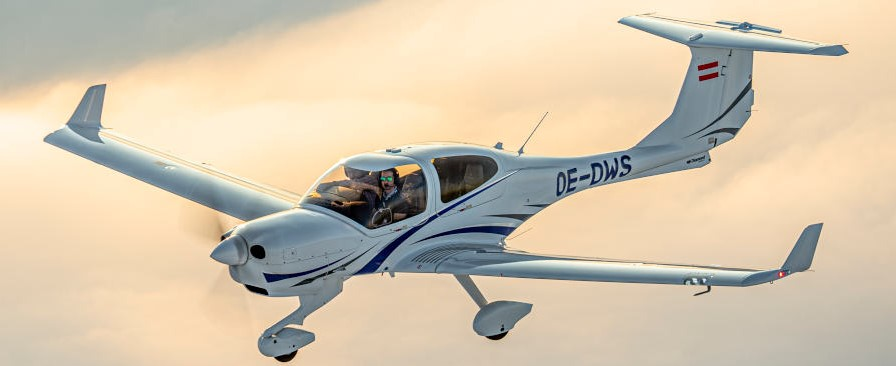
\includegraphics[width=.85\linewidth]{Figures/DA40.jpg}
    \caption{Pilot flying Diamond DA-40 single propeller aircraft~-~the focus of the collection platform for this thesis~\cite{DiamondAircraftDA40}.}
\end{figure}

\section{Reference Frames}
% What are reference frames
Reference frames and their transformations are a critical component to any navigation algorithm. Precise determination of a flight vehicle requires the knowledge of its position, velocity, and orientation. Reference frames describe the orientation of the flight vehicle in a global or local reference point. Because different components of the FVDM are physically located and oriented at unique locations of the Diamond DA-40, multiple reference frames are used to describe the forces and moments these components generate due to their placement. In order for the cumulative summation of all forces and moments generated at certain time step, reference frames transformation are used to coordinate local forces and moments into a congruent reference frame such that these calculations are performed properly. This section describes the different reference frames used in this work for the FVDM\@.
% The different reference frames on the aircraft model
% Body
\subsection{Flight Vehicle Reference Frame}\label{section:FVRF}
The flight vehicle reference frame or body frame describes the reference frame with origin at the center of mass of the modeled Diamond DA-40. The body frame maintains alignment shown in Figure~\ref{fig:flightvehiclereferenceframe} and remains fixed to the flight vehicle at all times. The flight vehicle reference frame is essential to the FVDM as all forces and moments are added together in the body frame before integration into global and local pose states.

\begin{figure}[!ht]
    \centering
    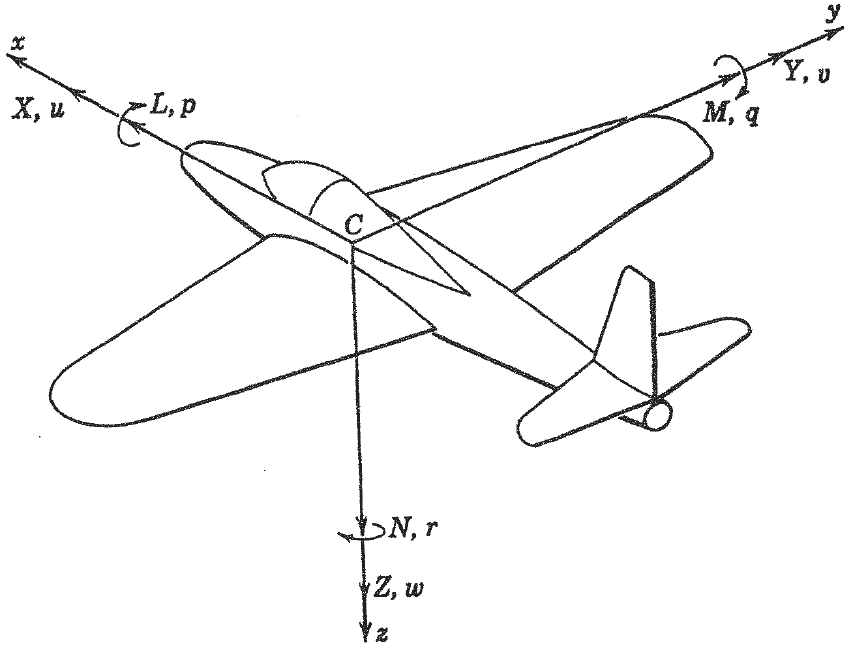
\includegraphics[width=0.60\linewidth]{Figures/bodyframe.png}
    \caption{Standard flight vehicle reference frame used in this work.~\cite{peetSpacecraftAircraftDynamics}}\label{fig:flightvehiclereferenceframe}
\end{figure}
\clearpage
% Prop
\subsection{Propeller Reference Frame}
The propeller reference frame describes the axis about which the propeller rotates with origin to the propeller nacelle, as seen in Figure~\ref{fig:propframe}. Propeller \textit{pitch}, as it is referenced in this thesis is a rotation about the \textit{y} axis, while the blades of the propeller rotate about the \textit{x} axis. This axis remains remains fixed in orientation and position (the frame origin being the propeller nacelle).~\( \phi{}\) from Figure~\ref{fig:propframe} describes the twist of the blade. The blade twist is a design choice of the propeller manufacturer. The twist of the blade helps the propeller produce more thrust, but is not used in any reference frame calculations.

\begin{figure}[!ht]
    \centering
    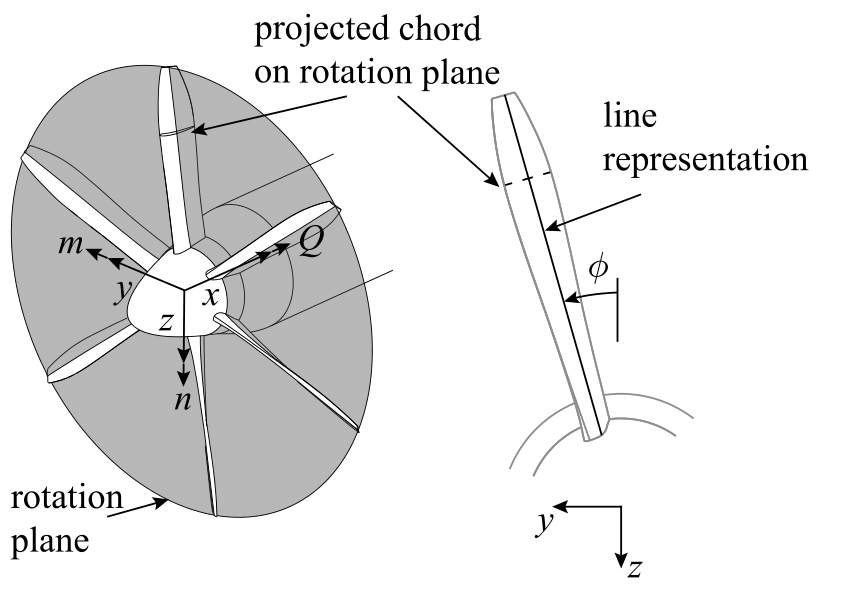
\includegraphics[width=0.75\linewidth]{Figures/propframe.png}
    \caption{The reference frame used to model the dynamic of the propeller in this work~\cite{vanarnhemEngineeringMethodEstimate2020}.}\label{fig:propframe}
\end{figure}

% Wind
\subsection{Local Wind Axes Reference Frame}
The local wind axes reference frame is used to calculate the lift and drag generated from their respective components with origin at the center of mass of the modeled Diamond DA-40. The orientation of the reference frame changes such that \(\Psi \) remains parallel with the trajectory of the aircraft and \(\alpha \) remains parallel to the ground below. In literature, \( \Psi \) and \(\alpha \) are referred to as the \textit{sideslip} and \textit{angle of attack} of the aircraft during flight.

\begin{figure}[!ht]
    \centering
    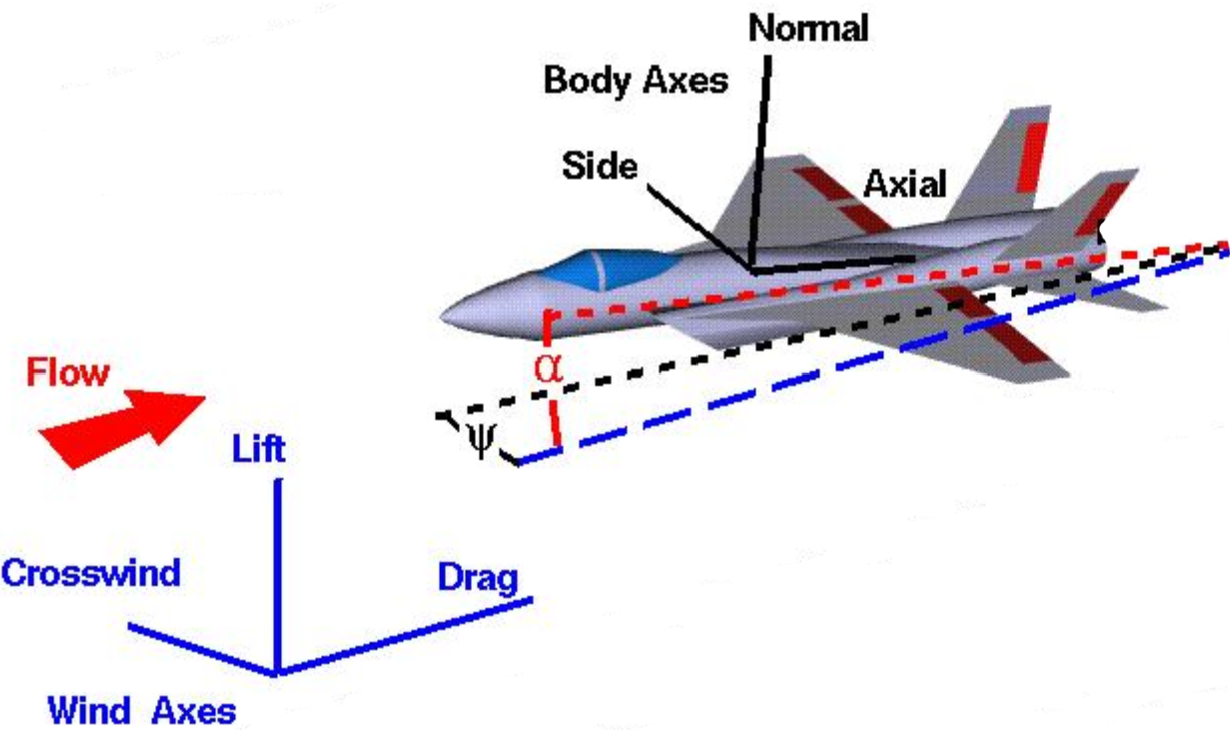
\includegraphics[width=0.75\linewidth]{Figures/windaxes.png}
    \caption{Flight vehicle reference frame and local wind reference frame (dotted lines) (Adapted from~\cite{ForceBalanceCoordinates}).}\label{fig:windframe}
\end{figure}

% Local
\subsection{Local Navigation Reference Frame}
A local navigation frame is necessary to define the orientation of the flight vehicle. This work implements a North-East-Down reference frame in which the axes are aligned with the topographic directions: North, East, and vertical as seen in Figure~\ref{fig:globalframes} by \(X_n\),\(Y_n\), and \(Z_n\). The origin of the local reference frame is defined at the initial position in the flight vehicle dynamics model and the navigation algorithm. The Euler attitude angles are used to describe the orientation of the Diamond DA-40 relative to the local navigation frame. When the aircraft has no roll pitch, or yaw, this equates to the aircraft flying perfectly tangential to Earth's ellipsoid, with the nose of the aircraft pointing towards the North.

\subsection{Global Reference Frames}
Global Reference Frames are critical for GPS receiver to calculate position and velocity. In summary, a position from a receiver is based on distances between the receiver and any visible satellites. As all GPS satellites operate in orbit around the Earth, the global reference frame provides a suitable solution that encompasses both satellite and receiver position and velocities. In this thesis, two global reference frames are used. The Earth-Centered, Earth-Fixed (ECEF) and the geodetic reference system. The ECEF reference frame is considered the standard global reference frame used as it works well for defining both positions and velocities for satellites and receivers, but falls short when it comes to visualization as the origin of the ECEF frame is the center of the Earth. The geodetic reference frame is an alternative frame that allows a visualization advantage by defining positions based on the surface of the Earth. Both LLA and ECEF reference frames utilize the World Geodetic System 1984 (WGS84) to describe Earth's geoid and gravitational field as function of parameters in Table~\ref{tbl:wgs84}. Visualization of both reference frames can be seen in Figure~\ref{fig:globalframes}.

\begin{table}[!ht]
    \caption{Properties describing the WGS84 ellipsoid}\label{tbl:wgs84}
    \centering
    \begin{tabular}{cccc}
        \toprule
        \textbf{Property}          & \textbf{WGS84 Value} & \textbf{Units} \\
        \midrule
        Equatorial Radius, \(R_0\) & 6,378,137.0          & meters         \\
        Polar Radius, \(R_P\)      & 6,356,752.31425      & meters         \\
        Flattening, \(f\)          & 1/298.257223563      &                \\
        Eccentricity, \(e\)        & 0.0818181808425      &                \\
        \bottomrule
    \end{tabular}
\end{table}

\begin{figure}[!ht]
    \centering
    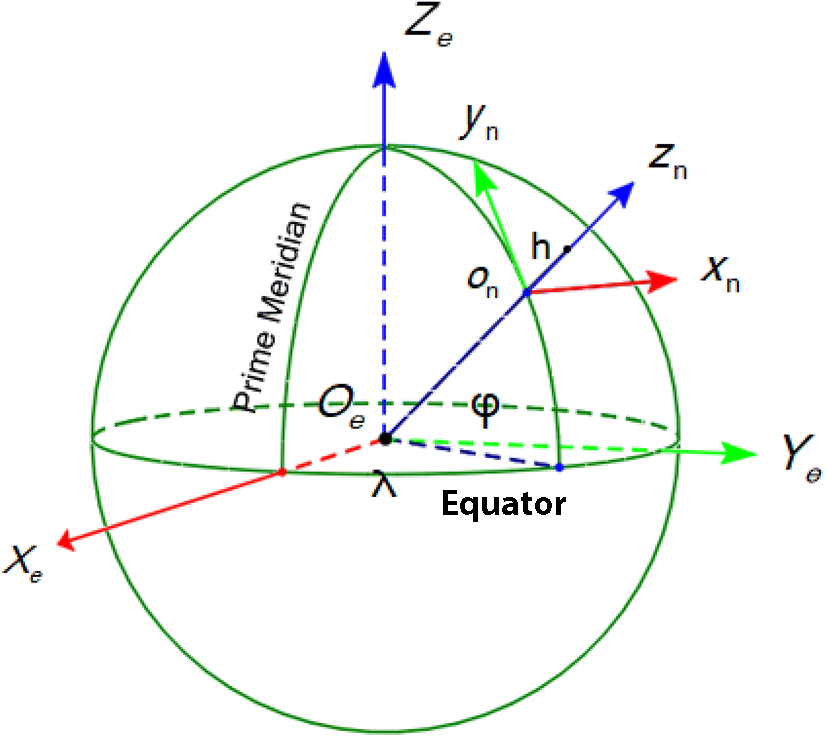
\includegraphics[width=0.75\linewidth]{Figures/globalframe.png}
    \caption{ECEF and geodetic reference frames as used in this thesis.}\label{fig:globalframes}
\end{figure}

% How the reference frames are calculated (DCMs)
\clearpage
\section{Reference Frame Transformations}
Reference frame transformations are critical to any sensor fusion algorithm in order to properly add vectors of different frames together. Reference frame transformations range in complexity, the simplest being a transformation of the NED frame into the East-North-Up reference frame. A more complex transformation could be the global ECEF frame into the body frame and vice versa. The reference frame transformation used in this thesis are described in the following subsections.

\subsection{ECEF to LLA}

One of the more complicated reference frame transformations is between the two global frames, ECEF and LLA\@. The conversion from LLA to ECEF is provided first in Equations~\ref{eq:meridiancurvature},~\ref{eq:transversecurvature},~\ref{eq:lla2ecefx},~\ref{eq:lla2ecefy}, and~\ref{eq:lla2ecefz}. The variables within these equations are defined in Table~\ref{tbl:wgs84}.

\begin{equation}\label{eq:meridiancurvature}
    R_N (L) = \frac{R_0 \, \left(1 - e^2\right)}{{\left(1 - e^2 \, \sin^2 {\left(L\right)}\right)}^{3/2}}
\end{equation}

Equation~\ref{eq:meridiancurvature}, \(R_N (L)\) describes the one the two radii of curvature. In this case, the meridian radius of curvature describes the north to south motion. The second radii of curvature (Equation~\ref{eq:transversecurvature}) describes the east to west motion and is known as the transverse radius of curvature (\(R_E (L) \)).

\begin{equation}\label{eq:transversecurvature}
    R_E (L) = \frac{R_0}{\sqrt{1 - e^2 \, \sin^2 {\left(L\right)}}}
\end{equation}

After the transverse radius of curvature is calculated, it used with the LLA positions to calculate the ECEF \(X\), \(Y\), and \(Z\) positions as shown in Equations~\ref{eq:lla2ecefx},~\ref{eq:lla2ecefy}, and~\ref{eq:lla2ecefz}.

\begin{equation}\label{eq:lla2ecefx}
    X_{ECEF} = \left(R_E (L) + h\right)\cos \left(L\right)\cos \left(\lambda\right)
\end{equation}

\begin{equation}\label{eq:lla2ecefy}
    Y_{ECEF} = \left(R_E (L) + h\right)\cos \left(L\right)\sin \left(\lambda\right)
\end{equation}

\begin{equation}\label{eq:lla2ecefz}
    Z_{ECEF} = \left[\left(1 - e^2\right) R_E (L) + h\right] \sin \left(L\right)
\end{equation}

The ECEF to LLA conversion is more complicated. In order to calculate \(L\) in Equation~\ref{eq:ecef2llaL}, \(h\) from Equation~\ref{eq:ecef2llaaltitude} must be calculated {--} and vice versa. The correct way to solve for positions in the LLA reference frame is iteratively until the difference between positions from iteration to iteration is miniscule.

\begin{equation}\label{eq:ecef2llaL}
    L = \textrm{atan2}\left(\frac{Z_{ECEF} \left[R_E (L) + h\right]}{\sqrt{X_{ECEF}^2 + Y^2_{ECEF}} \, \left[ \left(1 - e^2\right) R_E (L) + h\right]}\right)
\end{equation}

\begin{equation}\label{eq:ecef2llalambda}
    \lambda = \textrm{atan}\left(\frac{Y_{ECEF}}{X_{ECEF}}\right)
\end{equation}

\begin{equation}\label{eq:ecef2llaaltitude}
    h = \frac{\sqrt{X_{ECEF}^2 + Y^2_{ECEF}}}{\cos\left(L\right)} - R_E (L)
\end{equation}


\subsection{ECEF to Local}
The conversion from the ECEF reference frame to the local navigation reference frame can be done by forming a Direction Cosine Matrix (DCM),

\begin{equation}\label{eq:ECEF2LNDCM}
    C^{\textrm{LN}}_{\textrm{ECEF}} =
    \begin{bmatrix}
        -\sin\left(L\right)\cos\left(\lambda\right) & -\sin\left(L\right)\sin\left(\lambda\right) & \cos\left(L\right)  \\
        -\sin\left(\lambda\right)                   & \cos\left(\lambda\right)                    & 0                   \\
        -\cos\left(L\right)\cos\left(\lambda\right) & -\cos\left(L\right)\sin\left(\lambda\right) & -\sin\left(L\right) \\
    \end{bmatrix},
\end{equation}

and then multiplying the ECEF position vector to produce a position in the NED frame as discussed previously. In Equation~\ref{eq:ECEF2LNDCM}, \(C^{\textrm{LN}}_{\textrm{ECEF}}\) describes the DCM used for the transformation. The notation follows such that the subscript (ECEF) is the position in the original reference frame and the superscript (LN) is the reference frame the position is being rotated into. This thesis will always follow this notation to avoid any confusion.

\subsection{Local to Body}
Similar to the conversion of ECEF to the local navigation frame, the conversion from the local navigation to the flight vehicle reference frame can be done by forming the DCM (Equation~\ref{eq:321DCM}).
\begin{equation}\label{eq:321DCM}
    C^{\textrm{FV}}_{\textrm{LN}} =
    \begin{bmatrix}
        \textrm{c}_{\theta}\textrm{c}_{\psi}                                                        & \textrm{c}_{\theta}\textrm{s}_{\psi}                                                        & -\textrm{s}_{\theta}                 \\
        -\textrm{c}_{\phi}\textrm{s}_{\psi} + \textrm{s}_{\phi}\textrm{s}_{\theta}\textrm{c}_{\psi} & \textrm{c}_{\phi}\textrm{c}_{\psi} + \textrm{s}_{\phi}\textrm{s}_{\theta}\textrm{s}_{\psi}  & \textrm{s}_{\phi}\textrm{c}_{\theta} \\
        \textrm{s}_{\phi}\textrm{s}_{\psi} + \textrm{c}_{\phi}\textrm{s}_{\theta}\textrm{c}_{\psi}  & -\textrm{s}_{\phi}\textrm{c}_{\psi} + \textrm{c}_{\phi}\textrm{s}_{\theta}\textrm{s}_{\psi} & \textrm{c}_{\phi}\textrm{c}_{\theta} \\
    \end{bmatrix}
\end{equation}
In this case, the DCM comprises of the 3 Euler angles {--} roll (\( \phi \)), pitch (\( \theta \)), and yaw (\( \psi \)). To allow the matrix to fit the width of the paper, \textit{c} and \textit{s} denote the \textit{cosine} and \textit{sine} trigonometric functions, respectively.

If one wanted to convert position from the flight vehicle to ECEF reference frame, multiplying Equations~\ref{eq:321DCM} and~\ref{eq:ECEF2LNDCM} provides the user with a DCM to do this (Equation~\ref{eq:ECEF2BODY}).

\begin{equation}\label{eq:ECEF2BODY}
    C^{\textrm{FV}}_{\textrm{ECEF}} = C^{\textrm{FV}}_{\textrm{LN}} \, C^{\textrm{LN}}_{\textrm{ECEF}}
\end{equation}

It should be noted that any of these DCM reference frame transformations can be inverted by simply transposing the matrices.

\section{Atmosphere Model}\label{section:atmos}
In order to more accurately calculate a handful of dynamics models studied in this work, a model of Earth's atmosphere is needed to provided ambient temperature, pressure, density, speed of sound, and wind. This thesis uses the International Standard Atmosphere (ISA) model to approximate ambient temperature, ambient pressure, ambient density, and the speed of sound given a certain height above Mean Sea Level (MSL). Using an assumed linear distribution for temperature as a function of altitude, the ISA model assumes hydrostatic equilibrium as seen by Equation~\ref{eq:2.1},

\begin{equation}
    \frac{dP}{dh} = -\rho \, g,
    \label{eq:2.1}
\end{equation}

where \(\frac{dP}{dh}\) is the vertical pressure gradient as a factor of air density, \( \rho \), and Earth's gravity, \(g\). After integrating Equation~\ref{eq:2.1}, the ISA model uses the ideal gas law (Equation~\ref{eq:2.2})

\begin{equation}
    P = \rho \, R\textsubscript{air} \, T
    \label{eq:2.2}
\end{equation}

to solve for the ambient pressure \(P\), and density, \( \rho \). A complete form of the ISA model is seen in Equations~\ref{eq:2.3} and~\ref{eq:2.4}.

\begin{equation}
    P = P_0\,\exp\left({\frac{-g\,\Delta h}{R\textsubscript{air}\,T}}\right)
    \label{eq:2.3}
\end{equation}

\begin{equation}
    \rho = \rho_0\,\exp\left({\frac{-g\,\Delta h}{R\textsubscript{air}\,T}}\right)
    \label{eq:2.4}
\end{equation}

where \(P_0\) and \(\rho_0\) are atmospheric layer values for pressure and density, respectively; \(R\textsubscript{air}\) is the specific gas constant for air and \(\Delta h\) is difference between the current altitude of the flight vehicle and altitude of the current atmospheric layer. The speed of sound is a function of temperature and can be calculated using Equation~\ref{eq:2.5}

\begin{equation}
    a = \sqrt{\gamma \, R\textsubscript{air}\,T},
    \label{eq:2.5}
\end{equation}

where \(a\) is the speed of sound in meters per second and \( \gamma \) is the ratio of specific heats. Figure~\ref{fig:atmos} describes these atmospheric parameters from MSL to 85,000 meters above sea level.

Along with the aforementioned atmospheric parameters, wind is a vital modeling parameter for flight vehicles. For smaller SWAP flight vehicles, small gusts of wind can greatly affect their dynamics~\cite{raymerAircraftDesignConceptual2018}. This thesis uses an updated version of the Horizontal Wind Model~\cite{drobEmpiricalModelEarth2008,drobUpdateHorizontalWind2015} using collected satellite data from the Nation Oceanic and Atmospheric Administration (NOAA). The model accepts the current position of the flight vehicle to provide a predicted wind vector in the meridional and zonal reference frame. Implementation of the ISA model and calculation of winds can be found under \textit{Atmosphere.m} in~\cite{millerNsm0014thesis2023}.

\section{Aerodynamic Principles}\label{section:aerodynamic}
% Section Overview
In all phases of flight, the surfaces on any aircraft generate two aerodynamic forces {--} \textit{lift} and \textit{drag} along with an aerodynamic moment vector. Prior to the modern computer, these forces and moments were derived from swaths of wind tunnel~(Figure~\ref{fig:windtunnel}) data under various conditions. Today, during the research and development phase of modern production aircraft, these aerodynamics components can be determined using Computation Fluid Dynamic programs such as \textit{Flightstream}~\cite{FlightStream}. This subsections provides the modelling equations for the surfaces of the airplane that generate lift, drag and moments during simulation.

\begin{figure}[!ht]\label{fig:windtunnel}
    \centering
    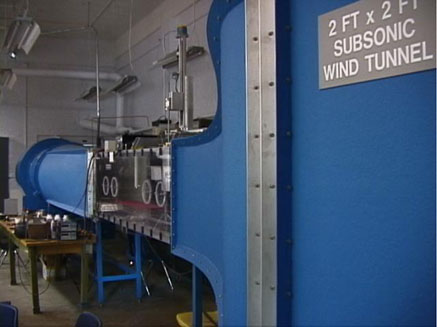
\includegraphics[width=.75\linewidth]{Figures/opencircuitwindtunnel.jpg}
    \caption{Subsonic wind tunnel in Auburn University's Aerodynamics Laboratory.}
\end{figure}

% How is lift generated?

A wing produces lift by allowing the air to move faster over the top of the airfoil. Bernoulli's principle equation (Equation~\ref{eq:bern})

\begin{equation}\label{eq:bern}
    P_1 + \frac{1}{2}\, \rho \, V_1^2 + \rho \, g \, h_1 = P_2 + \frac{1}{2}\, \rho \, V_2^2 + \rho \, g \, h_2
\end{equation}

shows that a fluid moving faster leads to a lower pressure gradient. On the bottom side of the wing, where the air is slower, a higher pressure gradient forms. This difference in pressure creates a force on the wing that lifts the wing and entire airplane into the air (Figure~\ref{fig:pressuregradient}).

\begin{figure}[!ht]\label{fig:pressuregradient}
    \centering
    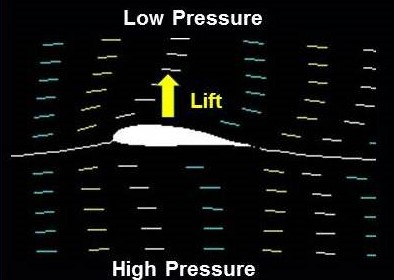
\includegraphics[width=0.75\linewidth]{Figures/foillift.jpg}
    \caption{Pressure gradient and subsequent lift produced onto an airfoil. The continuous white line in the middle signifies the freestream incident wind.}
\end{figure}

The lift generated by the wing (and subsequently the aircraft) can be calculated using Equation~\ref{eq:lift},

\begin{equation}\label{eq:lift}
    L = \frac{C_L \, \rho \, V^2 \, A}{2},
\end{equation}

where \(L\) is the lifting force, \(C_L\) is the lift coefficient for the aircraft or specific body, \( \rho \) is the density of fluid, \(V\) is the velocity of the fluid, and \(A\) is the surface area of aircraft or specific body. For the modelling and simulation of the Diamond DA-40 presented in this thesis, the aerodynamic coefficients are approximated using \textit{Strip Theory}.~\textit{Strip Theory} is covered in great detail later in this chapter.

% What is drag?
Lift is not the only force produced by the wing during flight. When any object moves through a fluid it produces drag. For the purpose of the modelling and simulation presented in this thesis, drag always opposes the aircraft's motion through air. Similar to Equation~\ref{eq:lift}, drag can be calculated using Equation~\ref{eq:drag}.

\begin{equation}\label{eq:drag}
    D = \frac{C_D \rho V^2 A}{2}
\end{equation}

The aerodynamic moments generated during flight of any aircraft are the single reason that control surface deflections cause the aircraft the roll, pitch or yaw in a certain direction. Just like the equations for lift and drag, the total aerodynamic moments is described in equation~\ref{eq:moment}.

\begin{equation}\label{eq:moment}
    M = \frac{C_M \rho V^2 A}{2}
\end{equation}

% What is Strip Theory?
In Equations~\ref{eq:lift},~\ref{eq:drag}, and~\ref{eq:moment}, coefficients need to be defined in order to calculate the aerodynamic forces and moments correctly. If known before hand, these coefficients can be calculated programmatically.~Equation~\ref{eq:CL} describes the equation for finding the lift coefficient.

\begin{equation}\label{eq:CL}
    C_L = C_{L_0} + C_{L_\alpha}\alpha + C_{L_q}\frac{qc}{2V} + C_{L_{\delta_e}}\delta_e
\end{equation}

Where \(C_{L_0}\) is the zero angle of attack lift coefficient, \(C_{L_\alpha}\) is the lift coefficient due to angle of attack, \(\alpha \) is the angle of attack,\(C_{L_q}\) is the lift coefficient due to the dynamic pressure, \(q\), and \(C_{L_{\delta_e}}\) is the lift coefficient due to the elevator deflection, \(\delta_e\).~\(c\) is the chord length of the wing and \(V\) is the speed of the aircraft. Equation~\ref{eq:CD} describes the equation for find the drag coefficient.

\begin{equation}\label{eq:CD}
    C_D = C_{D_0} + K\,C_{L}^2
\end{equation}

Where \(C_{D_0}\) is the zero angle of attack lift coefficient and \(K\) is the lift induced drag coefficient of the aircraft.

The aerodynamic moment coefficient is split into three components, each defined by the direction that act about the flight vehicle (described by Section~\ref{section:FVRF}). The rolling, pitching, and yawing moment are described by their respective Equations~\ref{eq:rollingmomentcoefficient},~\ref{eq:pitchingmomentcoefficient}, and~\ref{eq:yawingmomentcoefficient}.

\begin{equation}\label{eq:rollingmomentcoefficient}
    C_l = C_{l_\alpha}\alpha + C_{l_\beta}\beta + \frac{b}{2V}\left(C_{l_p}p + C_{l_r}r\right) + C_{l_{\delta_e}}\delta_e + C_{l_{\delta_a}}\delta_a + C_{l_{\delta_r}}\delta_r,
\end{equation}

\begin{equation}\label{eq:pitchingmomentcoefficient}
    C_m = C_{m_0} + C_{m_\alpha}\alpha + C_{m_\beta}\beta + \frac{c}{2V}\left(C_{m_{\dot{\alpha}}}\dot{\alpha} + C_{m_q}q\right) + C_{m_{\delta_e}}\delta_e
\end{equation}

\begin{equation}\label{eq:yawingmomentcoefficient}
    C_n = C_{n_\alpha}\alpha + C_{n_\beta}\beta + \frac{b}{2V}\left(C_{n_{p}}p + C_{n_r}r\right) + C_{n_{\delta_e}}\delta_e + C_{n_{\delta_a}}\delta_a + C_{n_{\delta_r}}\delta_r
\end{equation}

In the above equations, \(C_{{(.)}_{(.)}}\) are the coefficients relating to their respective aircraft states.~\(p\), \(q\), and \(r\) are the angular rates about the forward, right, and down direction in the flight vehicle reference frame.~\(\delta_e\), \(\delta_a\), and \(\delta_r\) are control surface deflections of the elevator, ailerons, and rudders, respectively.~\( \beta \) is the sideslip angle of the aircraft and represent the angle between the motion of the aircraft and the direction the aircraft is pointing. Finally, \(b\) describes the wing span of the aircraft.

Unless these coefficients and their accompanying variables are somehow known \textit{a priori}, determining what they should be can be cumbersome. However, one way to approximate the coefficients to their true value is to use a CFD program and collect tables of data for the aircraft under various flight condition and control surface deflections. The remaining part of this sections describes the process of using \textit{Flightstream} in combination with strip theory to closely mirror the true coefficient values.

For the aircraft model presented in this thesis, strip theory is a means to better approximate the lift, drag, and moments coefficients described earlier. Figure~\ref{fig:strips} draws the horizontal and vertical strips the aircraft is discretized into. Their reference frame is static and is defined by the strips position and orientation relative to the center of mass of the aircraft. To rotate the aerodynamic forces generated from each strip, a simple \( \psi-\theta-\phi \) transformation is used.

\begin{figure}[!ht]\label{fig:strips}
    \centering
    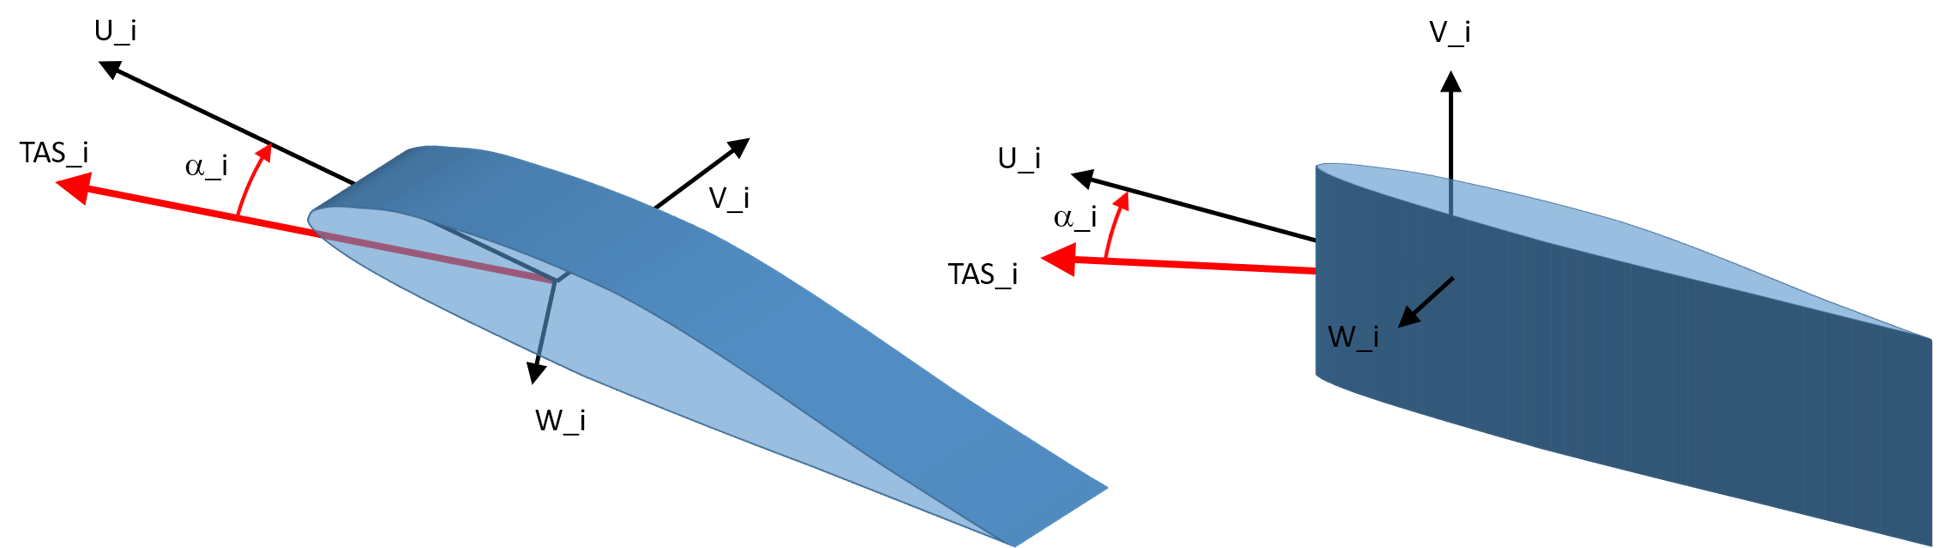
\includegraphics[width=0.75\linewidth]{Figures/horvertstrips.png}
    \caption{Horizontal and vertical strips that are analyzed for aerodynamic coefficients in FlightStream~\cite{AerodynamicStripTheory2021}.}
\end{figure}

Strip theory is a process in which a 3D model of the aircraft is discretized into independent strips and then processed through a CFD program to approximate the performance of the aircraft under various flight conditions. Flightstream~\cite{FlightStream} is used to generate aerodynamic coefficients for each strip. In Flightstream, the aircraft was evaluated on a range of angles of attack and sideslips, along with different control surface deflections. The aircraft was evaluated at a single velocity of 30 meters per second as the velocity component for the coefficient is just a scaling value.

Downwash is an aerodynamic property where the finite length of the lifting surfaces results in 3-dimensional flow fields causing reduction in effective angles of attack. To introduce downwash into the model and simulation, a reduced-ordered model utilizing integrated circulation was implemented~\cite{bhandariGeneticAlgorithmOptimization2023,ahujaIntegratedComputationalAeroacoustics2022}\@.

\section{Aero-Propulsive Forces}

Calculating lift, drag, and aerodynamic moments are useless unless the aircraft is moving. For any flight vehicle (except a glider), there is some form of engine or propeller that accelerates the incident freestream around the aircraft, allowing the lift, drag, and moment calculations to be of benefit. Similar to a ground vehicle, there is an infinite amount of complexity that can go into the modeling of a flight vehicles propulsion components. The work in this thesis focuses on the engine, shaft, and propeller {--} followed by the effects these components have on the aircraft. The following subsections describe the aero-propulsive flight mechanics that allow aircraft to accelerate, take off, and maintain altitude during the length of the flight.

\subsection{Piston Engine Model}
% Overview of Piston and Propeller Model
Small general aviation aircraft generate propulsive forces through use of an engine that spins a shaft which is connected to a propeller. The engine modeled and simulated is a piston, air-cooled engine. The typical aircraft piston engine is modeled as a four-stroke otto cycle~\cite{raymerAircraftDesignConceptual2018}. The otto cycle is a well-known thermodynamic theory that relies on a large air mass flow rate to generate power~\cite{gudmundssonGeneralAviationAircraft2014}. The components of the engine that produce the power are described below.

% Manifold Pressure
Because the engine is air-cooled, one of more important components is the engine manifold. The engine inlet manifold is a set of vents that allow the ambient air to feed directly into the combustion chambers where the oxygen in the air is used in combination with the fuel to generate power. Based on the commanded throttle input, these manifold vents can be closed or open to let in more or less air, and in return the engine delivers a proportional amount of power to the shaft. The power production from the engine is heavily reliant on the density of air. The Gagg and Ferrar model,

\begin{equation}\label{eq:gaggandferrar}
    \textrm{power} = \textrm{power}_{0}\left(\frac{\rho}{\rho_0} - \frac{1 - \rho/\rho_0}{7.55}\right),
\end{equation}

relates power production to the density of air. Where \(rho\) is the density of the ambient air as a function of altitude (Section~\ref{section:atmos}), \(rho_0\) is the density of ambient air at sea-level on a standard day, and \(\textrm{power}\) is the max engine power provided the density ratio and the nominal power production of the engine. From~\cite{hartzellpropellerHartzellPropellerManual2023}, the engine modeled in this work has a nominal power output on a sea-level standard day of 600 horsepower (447.42 kiloWatts). Figure~\ref{fig:gaggferrar} shows the power output of the engine modeled in this thesis based on the Gagg and Ferrar model and nominal sea-level power production.

\begin{figure}[!ht]\label{fig:gaggferrar}
    \centering
    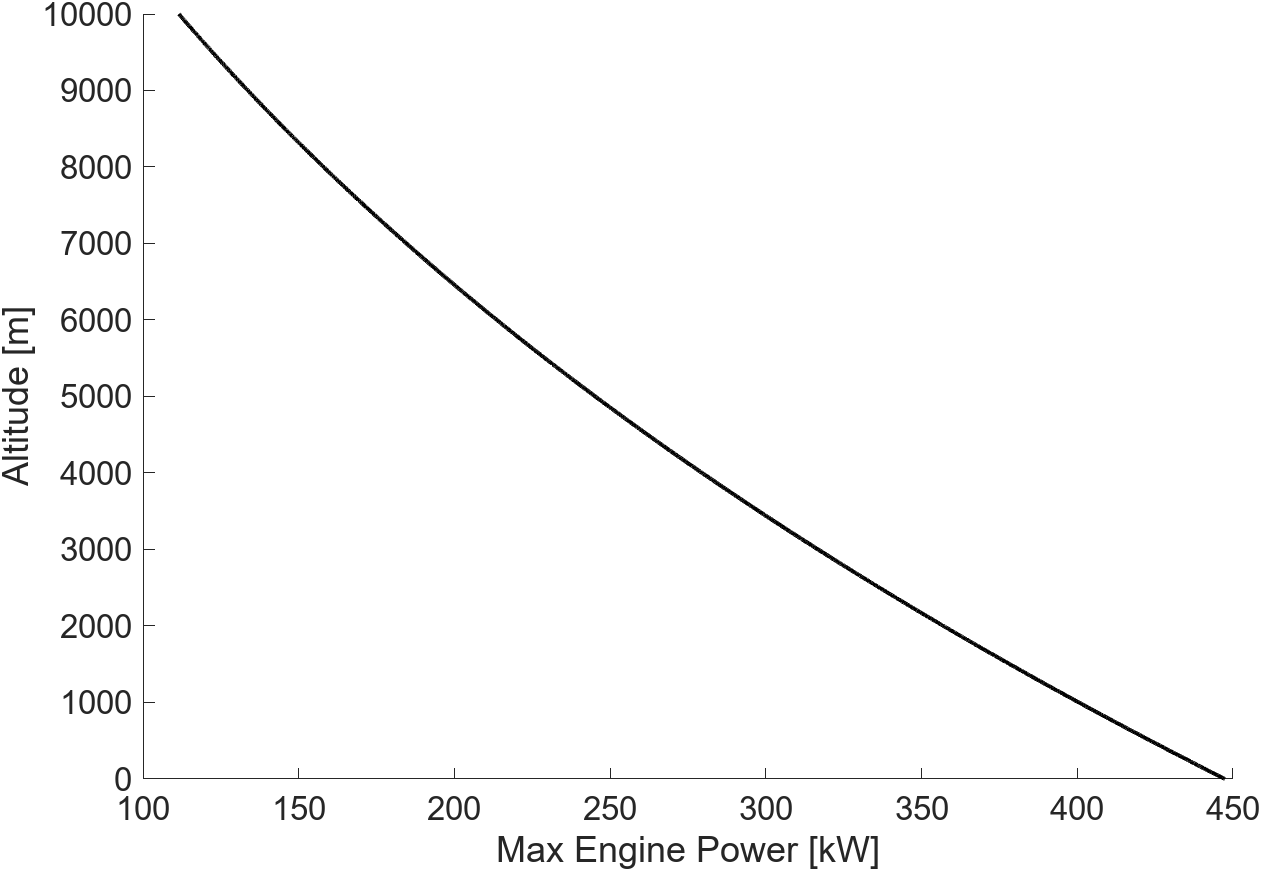
\includegraphics[width=0.85\linewidth]{Figures/gaggferrar.png}
    \caption{Power output for modeled engine as a function of aircraft altitude.}
\end{figure}

However, not all power generated by the engine is absorbed by the shaft. There are losses that include shaft slippage or uneven distribution of fuel in the combustion chamber. These \"errors\" are modeled as a \textit{Power Factor} and compares the the ideal power produced by the engine to the power absorbed by the shaft. This proportional amount is queried at every time step in the simulation as seen in Figure~\ref{fig:PFLUT}.

\begin{figure}[!ht]\label{fig:PFLUT}
    \centering
    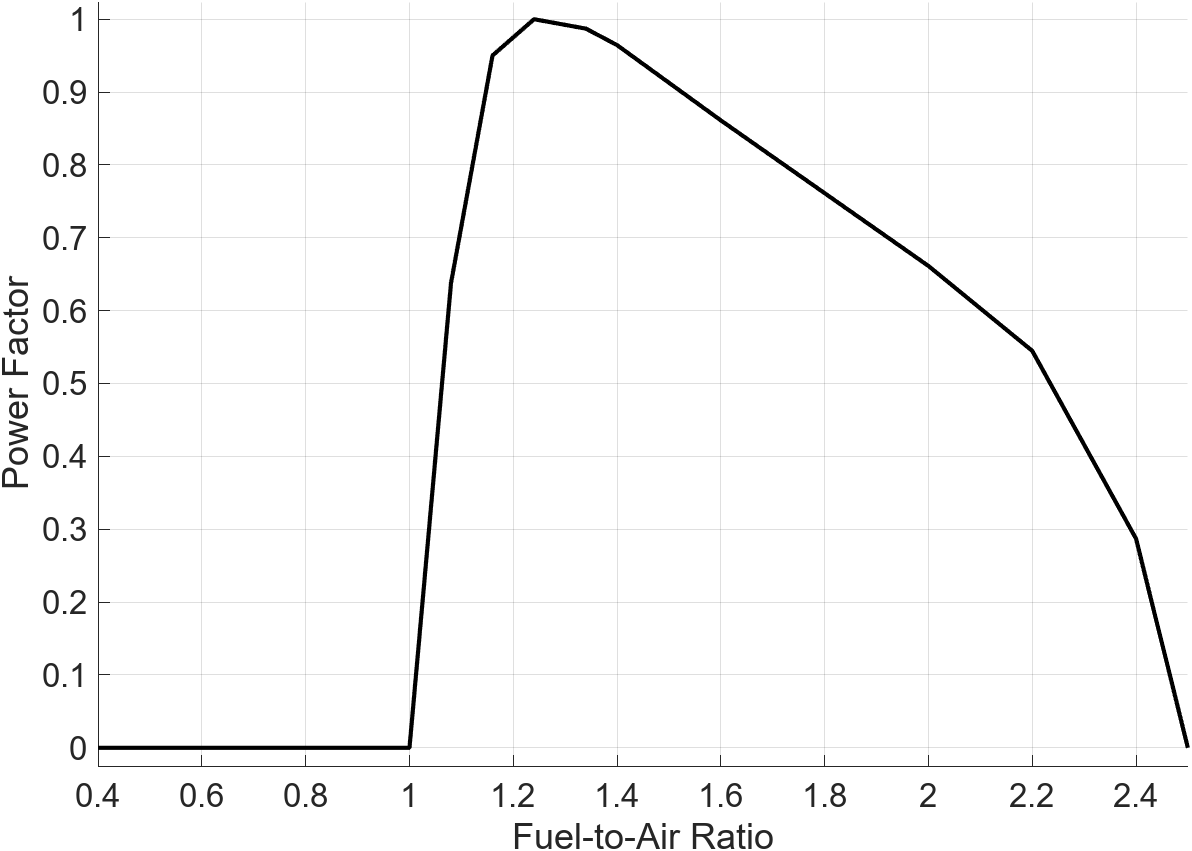
\includegraphics[width=.75\linewidth]{Figures/PFLUT.png}
    \caption{Power factor look up table for modeled engine.}
\end{figure}

% Electric Governor Model
The governor that exists in ground and flight vehicles exists such that drastic changes in throttle do not result in extreme ramps of torque that could structurally damage engine components. It limits the rate of commanded throttle to be linear so that rotational acceleration of the shaft and propeller is safely increased or decreased. The governor also controls fuel consumption of the engine by controlling the engine speed. The fuel consumption is queried at every time step using a look up table that is calculated before the simulation starts (Figure~\ref{fig:BSFCLUT}).

\begin{figure}[!ht]\label{fig:BSFCLUT}
    \centering
    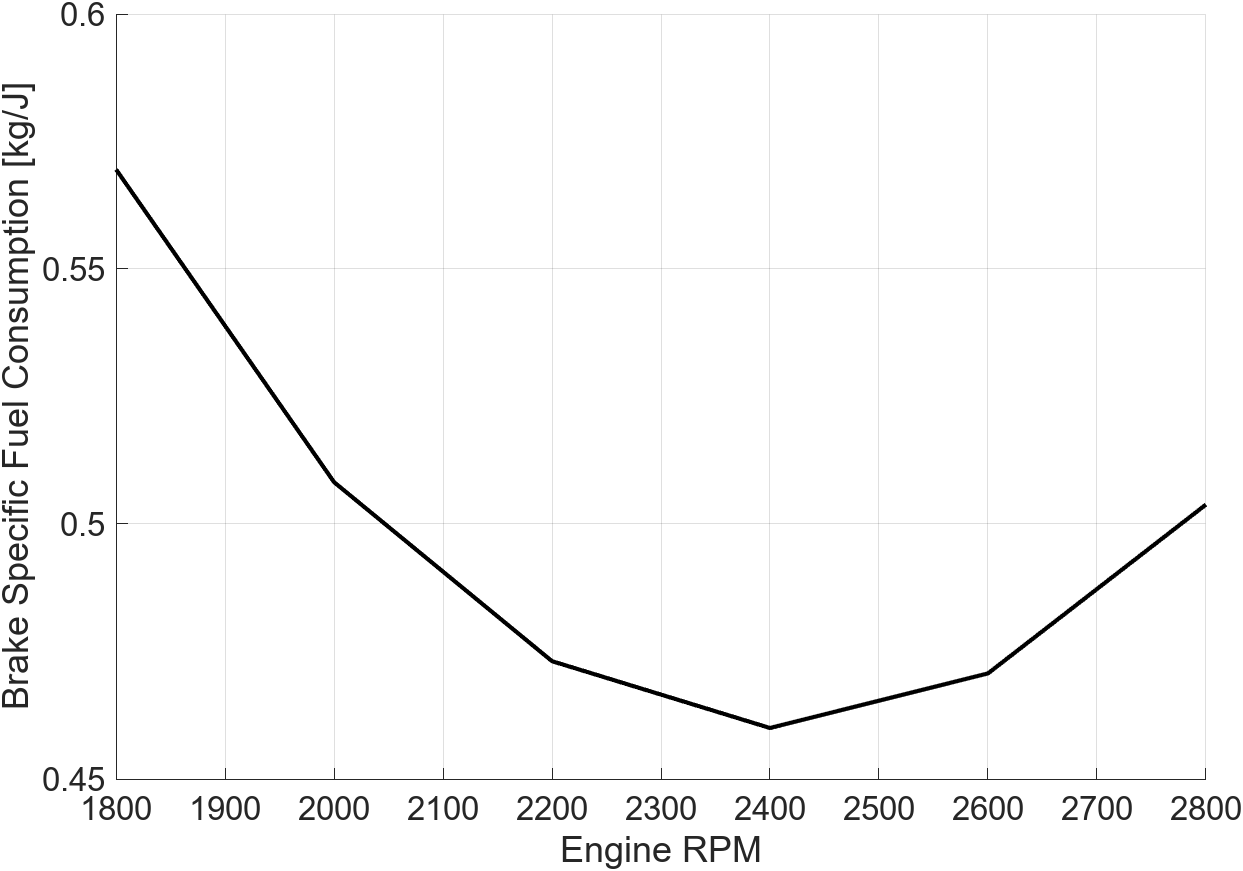
\includegraphics[width=.75\linewidth]{Figures/BSFCLUT.png}
    \caption{Brake specific fuel consumption look up table for modeled engine.}
\end{figure}

\subsection{Propeller Modeling}
% Propeller Dynamics
The purpose of an aircraft propeller is to increase the velocity of the ambient air around them such that the lifting surfaces on the aircraft can generate lift and keep the aircraft in flight. There are 3 main components to focus on when designing and manufacturing propellers. These are
\begin{itemize}
    \item[i.] Materials
    \item[ii.] Number of Blades
    \item[iii.] Blade Geometry.
\end{itemize}
While the focus of this thesis is not on details in propeller design, it is important to show how the history and differences between each of these 3 items affect the efficiency and performance a propeller has in generating thrust power for the aircraft. The first modern propeller were designed in the early 1900's. Originally made of wood, they featured 3 blades and crudely resembled airfoil shapes (Figure~\ref{fig:woodprops}).

\begin{figure}[!ht]\label{fig:woodprops}
    \centering
    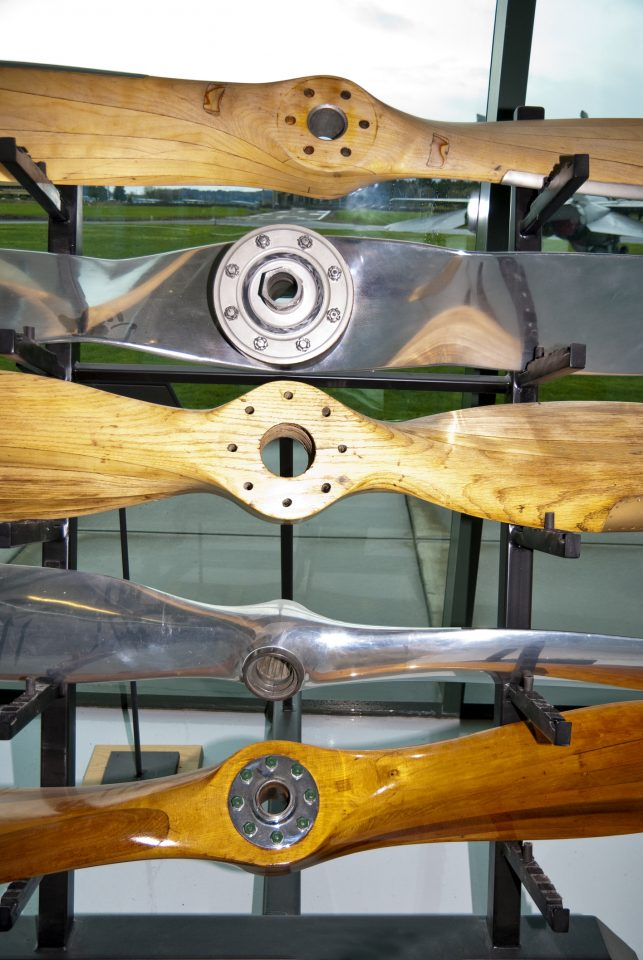
\includegraphics[width=0.3\linewidth]{Figures/woodProps.jpg}
    \caption{Collection of historic wood and steel propellers~\cite{ianHowIdentifyHistoric2016}.}
\end{figure}

These propellers had a fixed pitch, meaning they could not rotate up and down during flight~-~severely costing the propeller thrust power. In 1929, Wallace Turnbull invented the variable pitch propeller, allowing pilots to control the pitch the propeller, dramatically increasing propeller efficiency during flight~\cite{ianShortHistoryAircraft2018}. Through time and the advent of computers, Computational Fluid Dynamics (CFD) analyses shaped a handful of equations that define the performance and efficiency of a propeller design. In this work, a 3-blade Hartzell~\cite{HartzellPropellerInc} composite propeller is used as it is the Original Equipment Manufacturer (OEM) propeller on the Diamond DA-40 aircraft. This propeller is a variable-pitch constant speed propeller, meaning the pitch of the propeller is optimally adjusted for the current flight condition, while at the same time, maintaining a constant rotational speed to conserve fuel and hold a consistent propeller efficiency (Equation~\ref{eq:propellerefficiency}).

Before the simulation is started, the propeller is analyzed through \textit{FlightStream}~\cite{FlightStream}, a surface vorticity flow solver, to analyze the propeller for its lift coefficient (\(C_L\)) at varying flight conditions (Figure~\ref{fig:flightstreamprop}).

\begin{figure}[!ht]\label{fig:flightstreamprop}
    \centering
    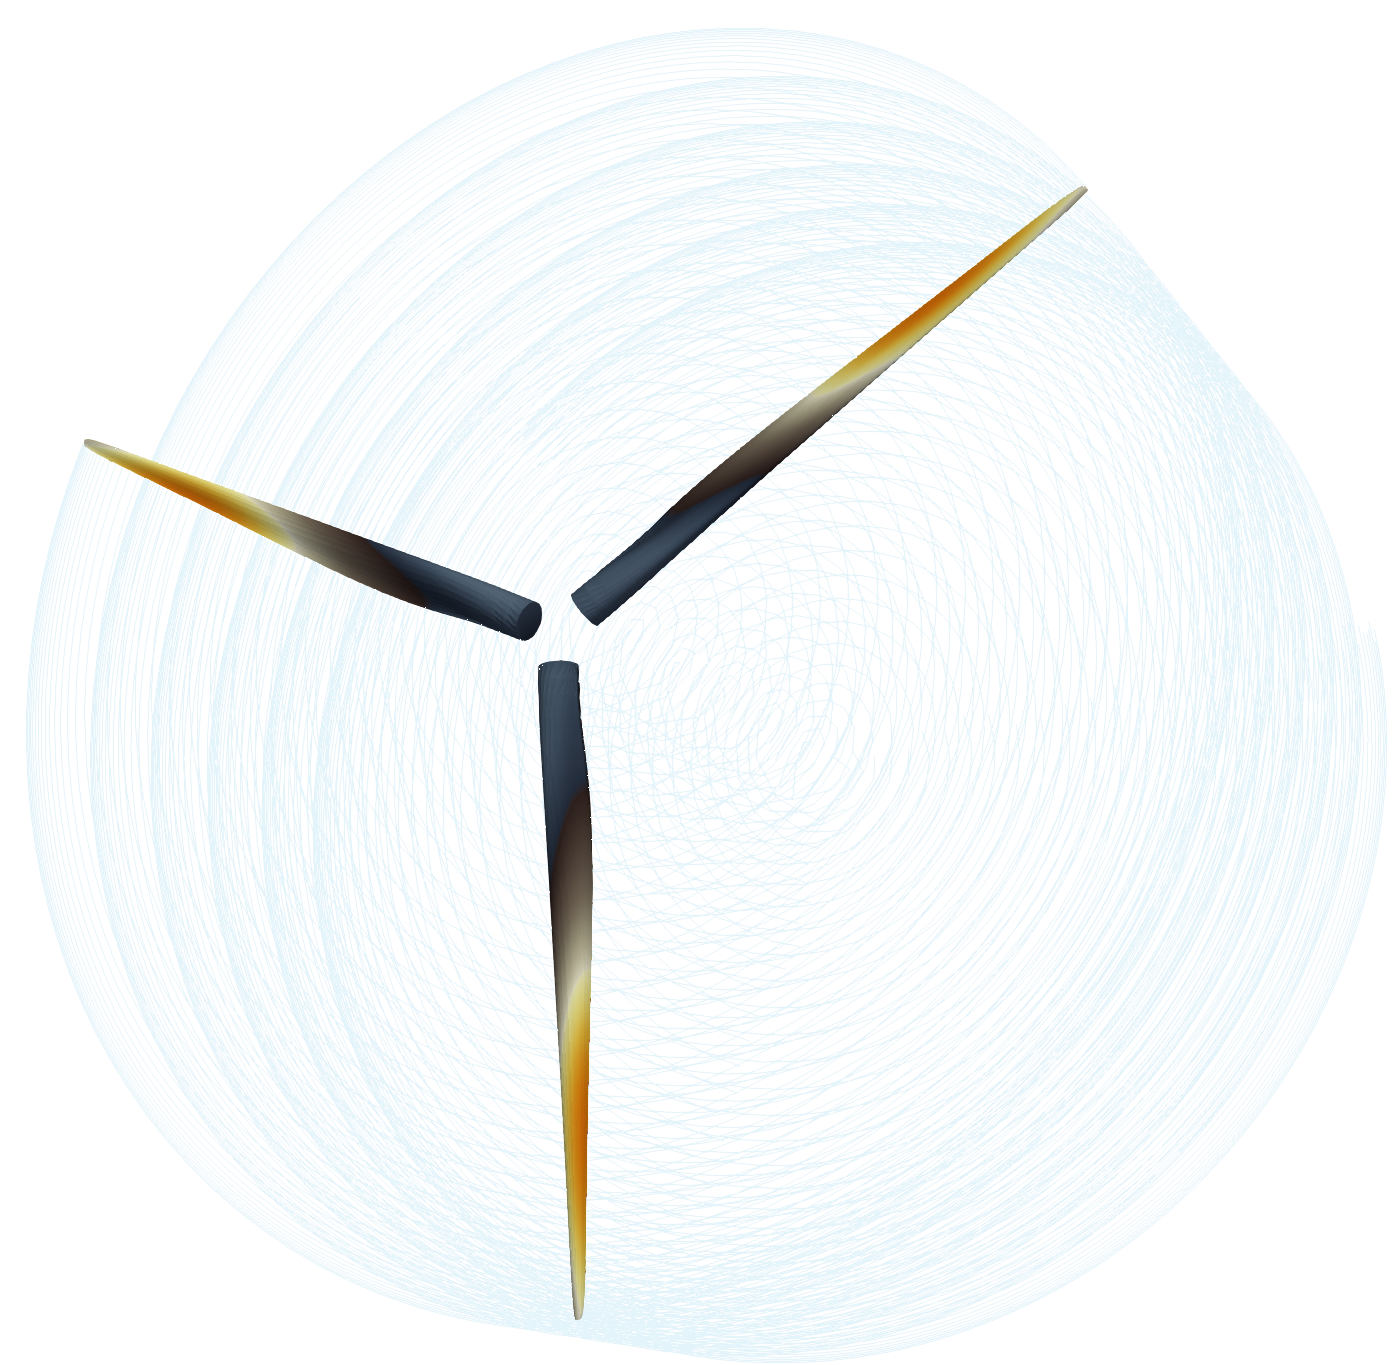
\includegraphics[width=.35\linewidth]{Figures/flightstreamprop.png}
    \caption{Analyzing 3-blade propeller through Flightstream~\cite{FlightStream}.}
\end{figure}

Once the lift coefficient is determined, numerical look up tables are generated such that the calculation of the forces and moments generated by the propeller can be interpolated, allowing the simulation to be run in real time. To determine the amount of thrust and torque generated by the propeller, the \textit{Activity Factor} (Equation~\ref{eq:activityfactor}) of the propeller must first be determined. The \textit{Activity Factor} is a measures of the propellers ability to absorb power and the effectiveness of each blade's width.

% Activity Factor
\begin{equation}\label{eq:activityfactor}
    AF_{\textrm{per blade}} = \frac{1 \times 10^5 \, c_{\textrm{root}}}{16 \, D} \left(0.25 + 0.2 \, \lambda - 0.2 \right)
\end{equation}

Where \(AF_{\textrm{per blade}}\) is the \textit{Activity Factor} per blade, \(c_{\textrm{root}}\) is the length of a blade's chord at the root, \(D\) is the diameter of the propeller, and \( \lambda \) is the taper ratio, described in Section~\ref{section:aerodynamic}. Table~\ref{tbl:propparams} describes the design characteristics of the propeller used in this thesis.

\begin{table}[!ht]\label{tbl:propparams}
    \caption{Characteristics of the propeller modeled for this work.}
    \centering
    \begin{tabular}{cccc}
        \toprule
        Characteristics       & Value  & Units  \\
        \midrule
        \(c_{\textrm{root}}\) & 0.1475 & meters \\
        \(D\)                 & 1.9    & meters \\
        \( \lambda \)         & 0.8    & N/A    \\
        \(C_L\)               & 0.5    & N/A    \\
        \bottomrule
    \end{tabular}
\end{table}

Because the dimensions of the propeller are known, we can determine the \textit{Activity Factor} of the blade to be (Equation~\ref{eq:activityfactorcalc},~\ref{eq:activityfactorcalc2})

% Activity Factor Calculation
\begin{equation}\label{eq:activityfactorcalc}
    AF_{\textrm{per blade}} = \frac{1 \times 10^5 \, (0.1475)}{16 \, (1.9)} \left(0.25 + 0.2 \, (0.8) - 0.2 \right)
\end{equation}

\begin{equation}\label{eq:activityfactorcalc2}
    AF_{\textrm{per blade}} = 101.89.
\end{equation}

Now that the \textit{Activity Factor} is known for the modeled propeller. The \textit{Power} (Equation~\ref{eq:powercoefficient}) and \textit{Thrust} (Equation~\ref{eq:thrustcoefficient}) coefficients can be calculated to show how well the propeller generates thrust when the aircraft is static (\i.e.\ starting takeoff). For this analysis, we assume the engine to be producing a nominal \(600\) horsepower (\(447.42\) [kW]) and applying a torque equivalent to \(2200\) [rpm] (\(36.6\) [rev\(/\)s]).

% Power Coefficient
\begin{equation}\label{eq:powercoefficient}
    c_P = \frac{P}{\rho \, n^3 \, D^5}
\end{equation}

% Thrust Coefficient
\begin{equation}\label{eq:thrustcoefficient}
    c_T = \frac{T}{\rho \, n^2 \, D^4}
\end{equation}

In Equations~\ref{eq:powercoefficient} and~\ref{eq:thrustcoefficient}, \(P\) is the engine power, denoted in kiloWatts, \(n\) is the rotational speed of the shaft, denoted in revolutions per second, \(T\) is the thrust of the propeller, denoted in kiloNewtons, and \( rho \) is density of the ambient air. For these calculations, an assume sea-level density is used (1.225 [\(kg/m^3\)]). Using Figure~\ref{fig:staticpropthrust} and our nominal engine power and torque output, we can approximate the thrust coefficient (Equations~\ref{eq:calcCT1},~\ref{eq:calcCT2},~\ref{eq:calcCT3} and~\ref{eq:calcCT4}).

\begin{figure}[!ht]\label{fig:staticpropthrust}
    \centering
    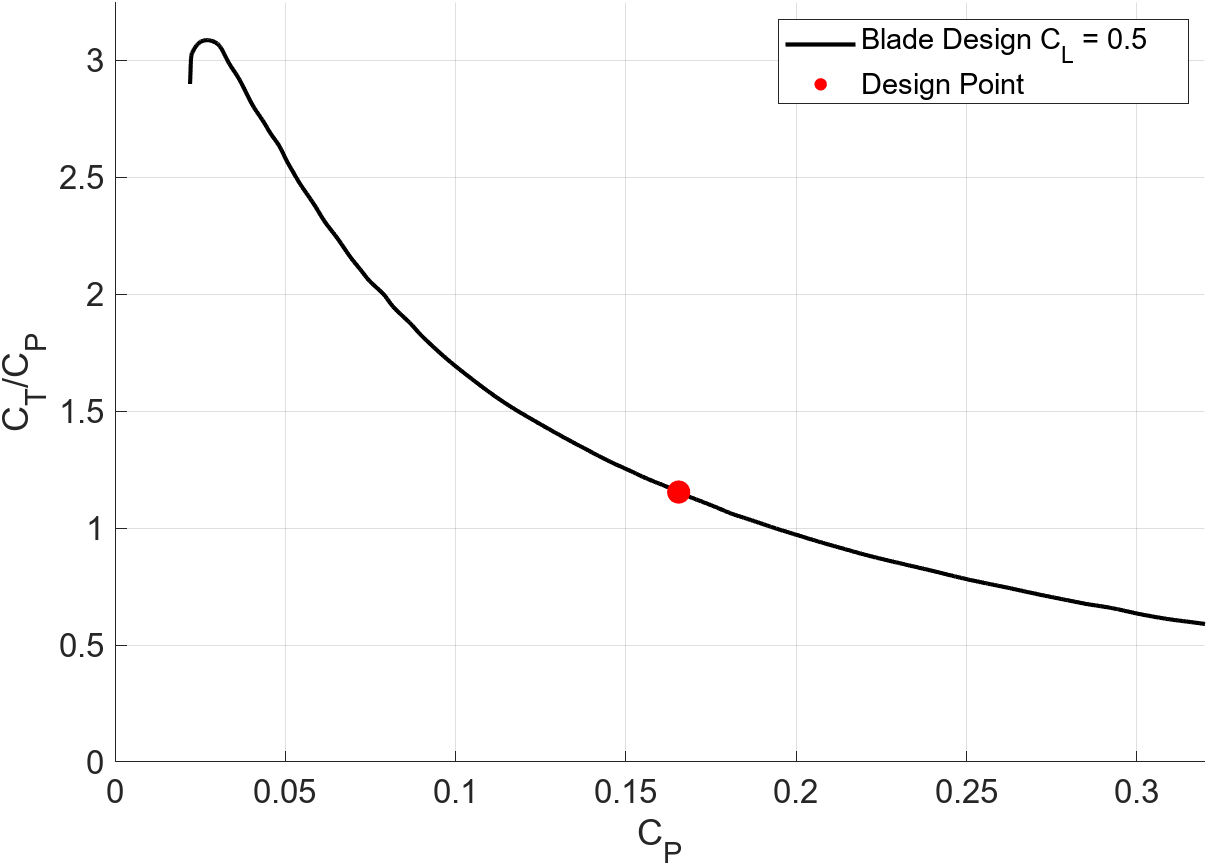
\includegraphics[width=0.85\linewidth]{Figures/StaticThrust.png}
    \caption{Static propeller thrust for the modelled propeller (Adapted from~\cite{GeneralizedMethodPropeller}).}
\end{figure}

\begin{equation}\label{eq:calcCT1}
    c_P = \frac{(447.42)(550)}{{(1.225)} \, {(36.6)}^3 \, {(1.9)}^5}
\end{equation}
\begin{equation}\label{eq:calcCT2}
    c_P = 0.16547
\end{equation}
\begin{equation}\label{eq:calcCT3}
    \frac{C_T}{C_P}(@C_P == 0.16547) = 1.1544
\end{equation}
\begin{equation}\label{eq:calcCT4}
    C_T = 0.18997
\end{equation}


Mapping \(C_T\) and \(C_P\) allows for computationally inexpensive queries with calculating propeller efficiency during flight (Equation~\ref{eq:propellerefficiency}).
% Propeller Efficiency
\begin{equation}\label{eq:propellerefficiency}
    \eta_P = \frac{C_T}{C_P} \, J
\end{equation}

Propeller efficiency, \( \eta_P \) compares the amount of power produced by the engine and shaft to the amount of power applied to the ambient air~-~an ideal propeller efficiency would be \(1\), where all of the produced engine power is used to accelerate the ambient air. The \textit{Advance Ratio}, \(J\)
% Advance Ratio
\begin{equation}\label{eq:advanceRatio}
    J = \frac{V}{n \, D} \, ,
\end{equation}

describes how far the flight vehicle moves at each full revolution of the propeller.
\(V\) is the forward velocity of the flight vehicle, \(n\) is the rotational speed of the propeller and \(D\) is the propeller diameter.

The final step in calculating the forces and moments generated by the propeller is querying the thrust based on the previous equations (Equation~\ref{eq:thrust}).
% Thrust
\begin{equation}\label{eq:thrust}
    T = \frac{P \, \eta_P}{V}
\end{equation}

A handful of steps, provided below, list the necessary calculations needed to simulate the thrust for the Diamond DA-40 modeled in this thesis. Because of some of the quantities are constant (i.e.\ propeller diameter and lift coefficient), look up tables can be created before hand to lower the computational load.

\begin{itemize}
    \item[1.] Calculate Activity Factor for given propeller design (Equation~\ref{eq:activityfactor}).
    \item[2.] Query coefficients data table (Figure~\ref{fig:staticpropthrust}) to define \textit{Power} and \textit{Thrust} coefficients (Equations~\ref{eq:powercoefficient} and~\ref{eq:thrustcoefficient}).
    \item[3.] Query \textit{Advance Ratio} (Equation~\ref{eq:advanceRatio}) data table for given flight velocity and shaft rotational speed.
    \item[4.] Calculate \( \eta_P \) (Equation~\ref{eq:propellerefficiency}), for given \(J\), \(C_P\), and \(C_T\).
    \item[5.] Calculate \(T\) using Equation~\ref{eq:thrust}.
    \item[6.] The moment generated by the propeller is simply the cross-product between the thrust and moment arm between the tip of the propeller and the nacelle of propeller.
\end{itemize}

\section{Landing Gear Model}
Although not calculated often, the modeling of the aircraft's landing gear are important and should not be overlooked. However, because of the flight paths investigated in this thesis focus solely on the aircraft during flight, a simplified dynamic model is used to describe the forces and moments acting on the landing gear during landing. It should be noted that the aerodynamic calculations of the landing gear occur in the aerodynamically modeling section, while this section focuses on the moments and forces generated from the runway opposing the weight of the aircraft.

To describe the forces and moments generated during landing, a mass-spring damper system (Figure~\ref{fig:ldgfbd}) can be used in simulate the the struts, levers, and tire depression (Figure~\ref{fig:ldg}) that absorb much of the forces, moments and vibrations that act onto the aircraft during landing.

\begin{figure}[!ht]\label{fig:ldgfbd}
    \centering
    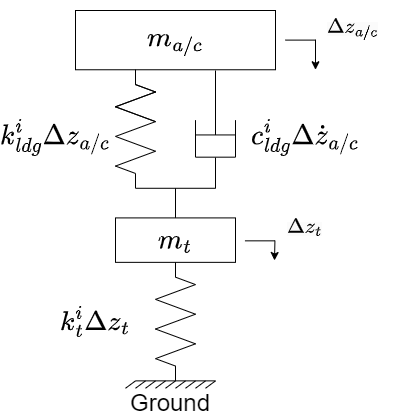
\includegraphics[width=.4\linewidth]{Figures/ldgfbd.drawio.png}
    \caption{Mass-spring damper system, representing the components of landing gear on the aircraft (adapted from~\cite{xingStrengthAnalysisDiagonal2012}).}
\end{figure}

\begin{figure}[!ht]\label{fig:ldg}
    \centering
    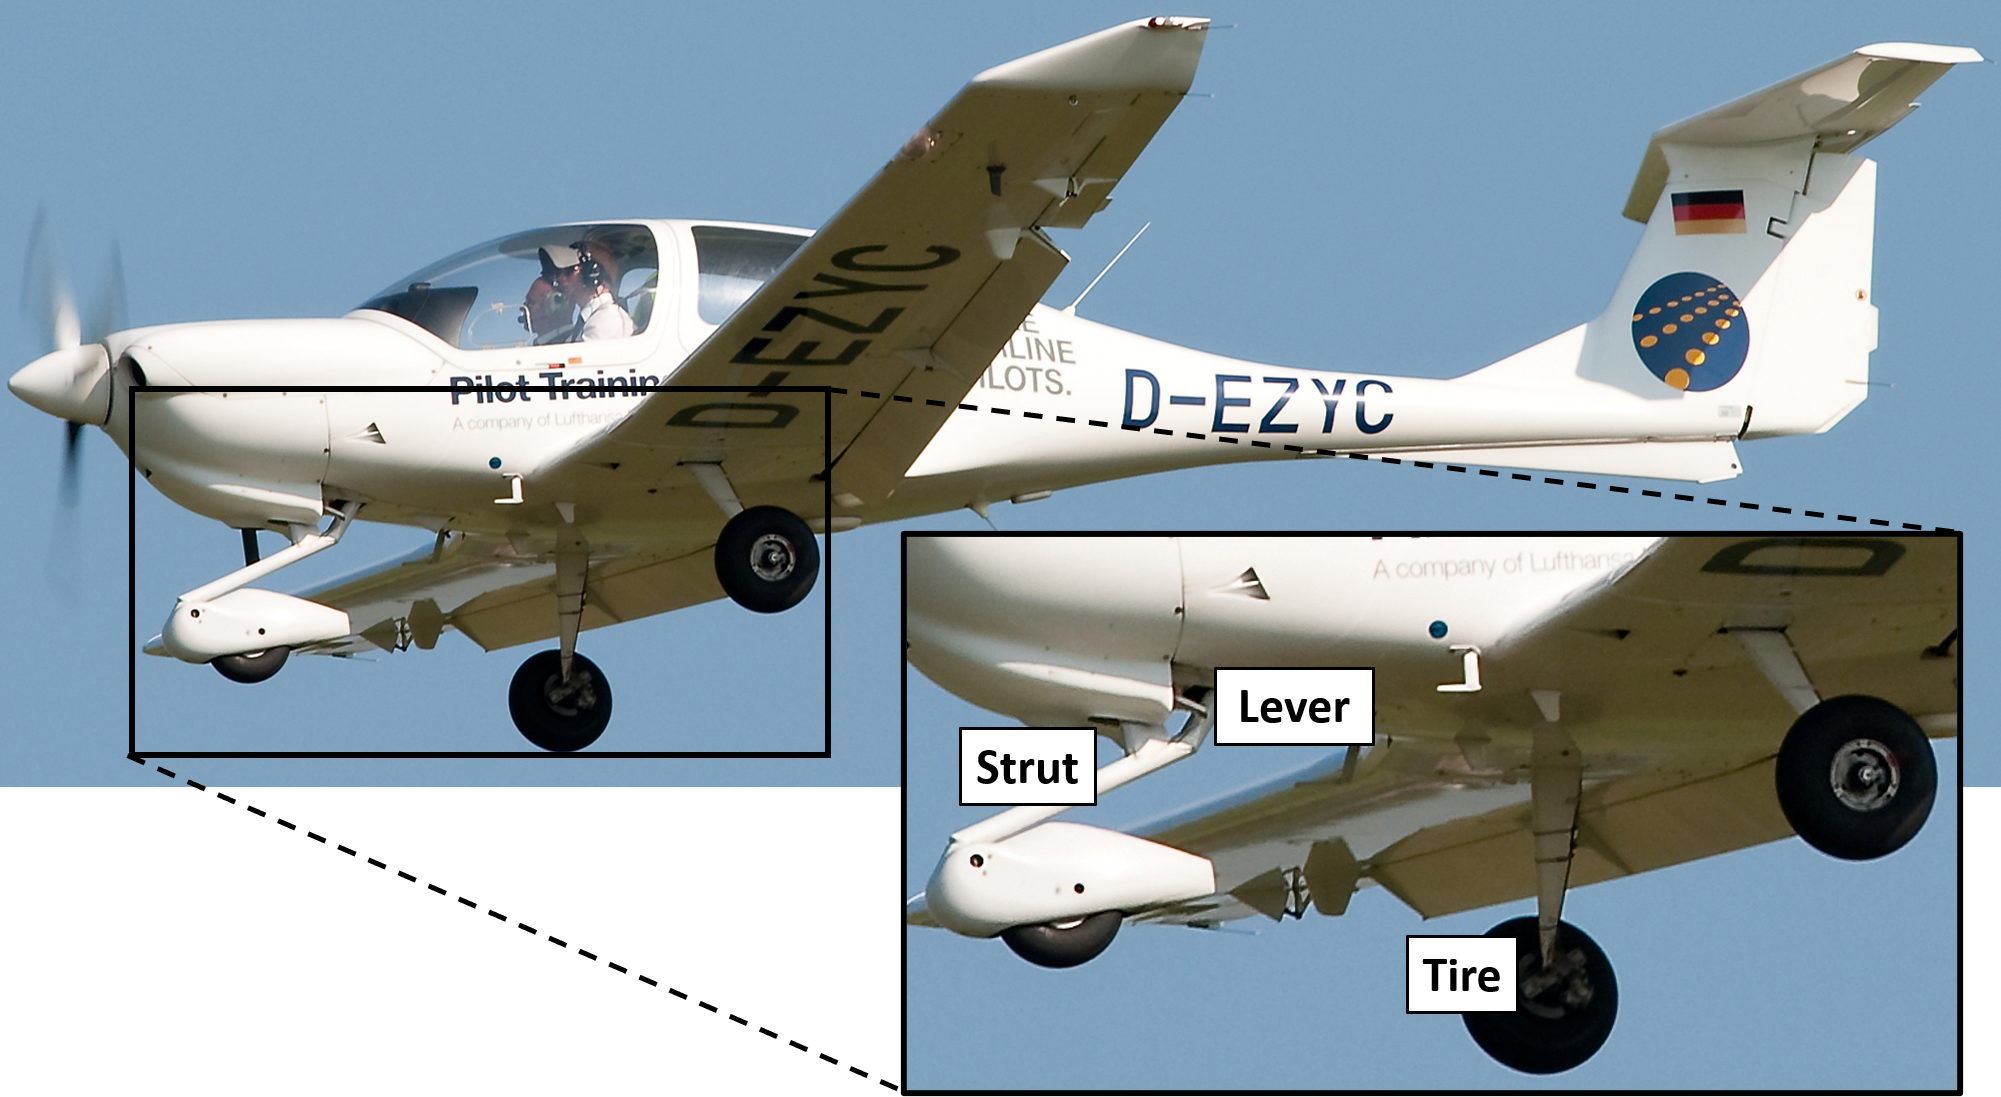
\includegraphics[width=.75\linewidth]{Figures/LandingGear.png}
    \caption{Identification of the landing gear components on the Diamond DA40.}
\end{figure}

Expanding Newton's second law, the forces on each landing gear are solved in the vertical direction (Equation~\ref{eq:ldgforces})

\begin{equation}
    \sum F^i_z = m\,a_z = k^i_t\, \Delta z_t\, + \, k^i_{ldg}\, \Delta z_{a/c}\, + c^i_{ldg}\, \Delta \dot{z}_t,
    \label{eq:ldgforces}
\end{equation}

where \(k^i_{ldg}\) and \(c^i_{ldg}\) are the spring and damper coefficients of the struts and levers respectively (see Table~\ref{tbl:ldgcoeff} for the values used in this simulated model). \(\Delta z_{a/c}\) and \(\Delta \dot{z}_t\), are the deflection and rate of deflection of the aircraft during landing.\( k^i_t \) and \(\Delta z_t\) are the tire \textit{spring} coefficient and tire depression respectively. For a general aviation aircraft, the depression of the tire upon landing is relatively small such that this term is thrown out.

\begin{table}[!ht]\label{tbl:ldgcoeff}
    \caption{List of spring and damper coefficients for nose and rear landing gear.}
    \centering
    \begin{tabular}{cccc}
        \toprule
        \textbf{i} & \textbf{Location} & \(\mathbf{k}\) \(  \left[\frac{kN}{m}\right]\) & \(\mathbf{c}\) \( \left[\frac{kN\,s}{m}\right]\) \\
        \midrule
        1          & Nose              & \(50\)                                         & \(11.3\)                                         \\
        2          & Rear Right        & \(80\)                                         & \(14.3\)                                         \\
        3          & Rear Left         & \(80\)                                         & \(14.3\)                                         \\
        \bottomrule
    \end{tabular}
\end{table}

The observed moments are solved by taking the cross product between the calculated forces of each landing gear and the moment arm (Equation~\ref{eq:ldgmoments}).

\begin{equation}
    \sum M^i = \textnormal{cross}([\,0\,;\,0\,;\,F^i_z\,],[\,x^i\,;\,y^i\,;\,z^i\,])
    \label{eq:ldgmoments}
\end{equation}

In Equation~\ref{eq:ldgmoments}, \(x^i\), \(y^i\), and \(z^i\) represent the moment arm that is derived from the center of gravity for the aircraft down to where each tire makes contact with the ground.

As a final note, it should be made clear that the forces and moments that act upon the landing gear if and only if a tire has made contact with the ground.

\section{Forces and Moments Calculations}
The final product of the aforementioned systems sums to 2 things~-~the forces and moments acting on the body of the aircraft. This work demonstrates the high-fidelity modelling of engines, propellers, landing gear, and aerodynamic forces and moments the simulated flight vehicles generates while in flight. The final step of these calculations is to add them together in the body-fixed \(X\), \(Y\), and \(Z\) directions. This is demonstrated by Equation~\ref{eq:sumForce} and Equation~\ref{eq:sumMoments}.

\begin{equation}
    \sum \mathbf{F} = \mathbf{F}_{prop} + \mathbf{F}_{aero} + \mathbf{F}_{LDG}
    \label{eq:sumForce}
\end{equation}

\begin{equation}
    \sum \mathbf{M} = \mathbf{M}_{prop} + \mathbf{M}_{aero} + \mathbf{M}_{LDG}
    \label{eq:sumMoments}
\end{equation}

It should be noted that \(\mathbf{F}_{LDG}\) and \(\mathbf{M}_{LDG}\) are only calculated when the aircraft is landing.

Once the forces and moments are calculated, they are used within the equation of motions that propagate the position, velocity, angular rates, and orientation in time during the simulation of the flight.

\section{Conclusions}

This section provided an overview of the reference frames used heavily when calculating the forces and moments the airframe of the aircraft experiences during flight. Following a discussion of reference frames, the ISA atmospheric model used in this work was defined with accompanying equations. The bulk of this chapter contains information about the use of strip theory for modelling the aerodynamics of the aircraft and a discussion of the engine and propeller modelling that produces the thrust for the Diamond-DA40 during flight. This chapter concludes with a description of the landing gear model and the summation of the forces and moments generated from the aforementioned sections that will be used in the equations of motions. Because the equations of motions are embedded within the proposed navigation filter for this work, they will be discussed in chapter 4. 
\clearpage